%!TEX program = xelatex
\documentclass[tikz, border=3pt]{standalone}  % 核心配置:独立画布+智能裁剪
\usepackage{pgfplots}
\usepgfplotslibrary{colormaps}
\pgfplotsset{compat=1.18}

\begin{document}
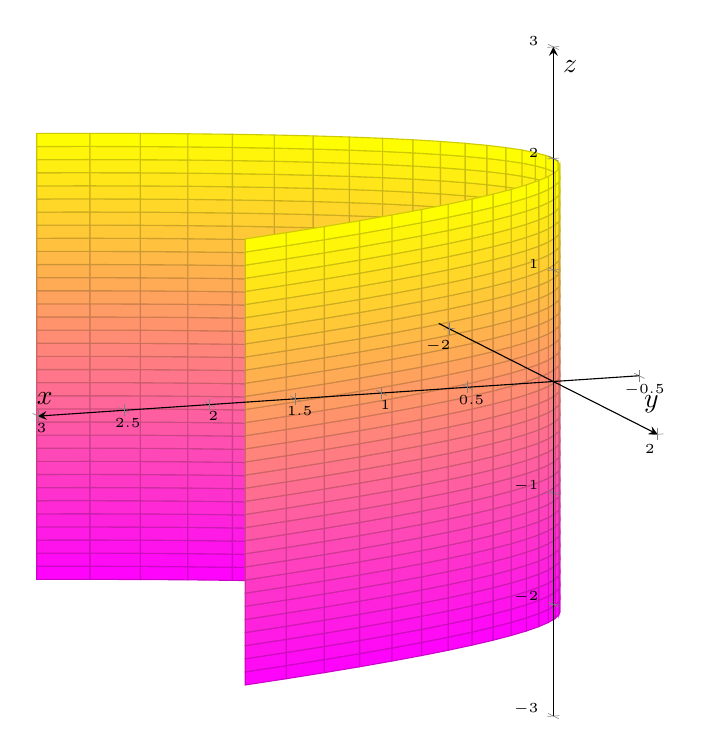
\begin{tikzpicture}
    \begin{axis}[
        colormap/spring,                    % 颜色映射声明移至axis环境
        view={160}{10},
        axis lines=center,
        axis on top,
        xlabel={$x$}, ylabel={$y$}, zlabel={$z$},
        xmin=-0.5, xmax=3,                  % 显式设置x最小值(因0.6x²≥0)
        ymin=-2.2, ymax=2,                  % 扩展y轴显示范围
        zmin=-3, zmax=3,
        width=12cm, height=12cm,
        tick label style={font=\tiny}
    ]
        \addplot3 [
            surf,
            z buffer=sort,
            samples=35, samples y=35,       % 均衡采样密度
            domain=-2:2,
            y domain=-2:2
        ] ({0.6*x^2},{x},{y});              % 抛物柱面参数方程
    \end{axis}
\end{tikzpicture}
\end{document}
